
\section{Goals For This Thesis}
This work focuses on providing a number of implementations of a Generative Chatbot, installed on small headless computers. Some overall goals are listed below. Checks in the check-boxes indicates the goal was achieved.

\begin{itemize}
	
	\item[\rlap{\raisebox{0.3ex}{\hspace{0.4ex}\tiny \ding{52}}}$\square$] Implement a generative chatbot using Recurrent Network components. This implementation uses GRU objects and the Tutorial found at Inkawhich et al \cite{2018Inkawhich}.
	
	\item[\rlap{\raisebox{0.3ex}{\hspace{0.4ex}\tiny \ding{52}}}$\square$] Implement a generative chatbot using a Transformer architecture and the Movie Dialog Corpus. This is discussed in Section \ref{transformer-movie-corpus}. %This implementation uses Scaled Dot Product attention.
	
	\item[\rlap{\raisebox{0.3ex}{\hspace{0.4ex}\tiny \ding{52}}}$\square$] Implement a chatbot using the Generative Pre-Trained 2 transformer. This is a pre-trained model. This is discussed in Section \ref{install-gpt2-chatbot}.
	
	\item[\rlap{\raisebox{0.3ex}{\hspace{0.4ex}\tiny \ding{52}}}$\square$] Subjectively compare the GRU, Transformer, and GPT2 models and the kind of output that each one produces. This is discussed throughout Section \ref{experiments-installations}.
	
	\item[\rlap{\raisebox{0.3ex}{\hspace{0.4ex}\tiny \ding{52}}}$\square$] Successfully install Google Speech Recognition and Text To Speech on the Raspberry Pi computer platform, as well as other small computers like the NVIDIA Jetson Nano. This is discussed in Section \ref{speech-and-speech-to-text}.
	
	\item[\rlap{\raisebox{0.3ex}{\hspace{0.4ex}\tiny \ding{52}}}$\square$] Install a GRU, Transformer, and GPT2 model on individual Raspberry Pi computers. Also install Google Speech Recognition and Speech To Text on these computers so that they can operate without keyboard or monitor. Allow the chatbot model to interact with a human's voice. This is discussed throughout Section \ref{experiments-installations}.
	
	\item[\rlap{\raisebox{0.3ex}{\hspace{0.4ex}\tiny \ding{52}}}$\square$] Install a GPT2 model on a Jetson Nano, along with Google Speech libraries and allow a human to interact with the chatbot. Compare execution time to the same model on the Raspberry Pi. This is discussed in Section \ref{chapter-nano}.
	
	\item[\rlap{\raisebox{0.3ex}{\hspace{0.4ex}\tiny \ding{52}}}$\square$] Compare the GRU and the Transformer model. Try to compare the word usage and sentence usage of the GRU and Transformer. This is discussed in Section \ref{gru-vs-transformer}.
	
	\item[\rlap{\raisebox{0.3ex}{\hspace{0.4ex}\scriptsize \ding{56}}}$\square$] Implement a generative chatbot using Recurrent Network components and an independent code base. This was not accomplished.
	
	\item[\rlap{\raisebox{0.3ex}{\hspace{0.4ex}\scriptsize \ding{56}}}$\square$] Implement a generative chatbot using a Transformer architecture and the Persona chatbot corpus. This implementation did not work well. This is discussed in Section \ref{transformer-persona-corpus}. %uses Scaled Dot Product attention.
	
	\item[\rlap{\raisebox{0.3ex}{\hspace{0.4ex}\scriptsize \ding{56}}}$\square$] Experiment with the GPT3 code. This was not accomplished. This is discussed in Section \ref{discussion-gpt3}.
\end{itemize}


\section{GRU vs. Transformer}
\label{gru-vs-transformer}

The GRU chatbot was compared with the larger Transformer based chatbot. Using subjective qualifications the GRU model answered accurately and with more variety than the Transformer model. An important observation was that the hyper-parameter set for the Transformer model could be expanded and enlarged as needed before training. The GRU model could not be trained successfully with an arbitrarily large hyper-parameter set. The larger Transformer could be trained to produce better responses.

Additionally, the GRU model responded very quickly, while the Transformer model took longer. The time spent by the Transformer model when installed on a small computer like a Raspberry Pi could not be ignored. 

Furthermore, time complexity is discussed by Vaswani et al \cite{Vaswani2017AttentionIA}. 
For the GRU Recurrent Neural Network it is $ n \cdot d^2 $, where $ n $ is the number of words in a sentence and $ d $ is the dimension of the hidden vector. Complexity for the Transformer's Scaled Dot Product Attention is $ n^2 \cdot  d $. Again, $n$ is the number of words and $d$ is the hidden vector's dimension. 

The maximum allowable input from the GRU is short, and in the example was 10. The maximum allowable input from the Transformer models varies but, in the 117M GPT2 model, it was 1024. 


In this example, the hidden vector size for the GRU model was 500 and %. The size for the 117M GPT2 model was 768, and 
the Transformer's hidden size was 512.

\section{Turing Test}

The Turing Test concerns itself with the question of whether a computer is intelligent. Turing says that intelligence is too hard to describe and that, if the computer can convince you that it is intelligent, then it is.

Whether this is right is beyond the scope of this thesis. The developers of the Generative Pre-Training 2 transformer were apprehensive about their model's ability to generate human-like text and felt the model worked too well. 
At first they decided not to release the largest version to the public for several months. 
They felt that the model could be used to spam Facebook and other social networking sites with content that was very convincing. 


Ultimately the large model was released, possibly because the developers decided the model was not as good as originally estimated. %, or because they didn't care. 

\section{Word and Sentence Comparisons}

It is important to understand the training and inference stages. Several graphs and a discussion of the GRU model and the Transformer model and their word and sentence usage follows.

The fully trained GRU and Transformer models are set up in inference mode and their output is observed when they are exposed to the first 100,000 training question sentences from the Movie Subtitles corpus.

All the graphs start out with one of the network models and a group of 100,000 input sentences. With every change of $x$ all the sentences up until that index are fed to the model. Then they are processed by whether or not they show up repeatedly in the output so far. Then the output is summed. The changes in $y$ show this summed output.

\subsection{Word Usage}

In general the Transformer model uses only a small subset of words that it has available to it. In the example below, Figure \ref{diagram-words-with-voc-total}, 100,000 input lines were tested from the training set. A small percentage of the vocabulary words were used in the output. %These sentences came from the movie dialog corpus. Some percentage of words are used repeatedly.

The graph in Figure \ref{diagram-words-with-voc-total} uses all three chatbot models. The graph uses 100,000 sentences from the Movie Dialog corpus, but from these question/answer pairs only the question is needed. Each question in turn is fed to each of the models. The output in terms of `Word Responses' is totaled at each $x$ index for the GPT2, the Transformer, and the GRU. For each $x$, the $y$ on the graph represents a running total showing how many words the model uses in its output. Pictured in this graph is also the `Total Vocabulary' number for the GPT2 model and the `Total Vocabulary' for the GRU model.

\begin{figure}[H]
	\begin{center}
		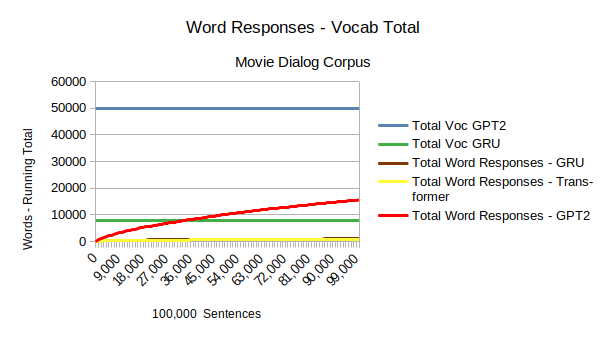
\includegraphics[scale=0.75]{diagram-100000-vocab}
		
		
	\end{center}
	\caption[Word Usage]{Word Usage - Including Vocabulary Total}
	\label{diagram-words-with-voc-total}
	
\end{figure}

The blue line at the top of Figure \ref{diagram-words-with-voc-total} is the total words in the GPT2 vocabulary. It is much higher than the GRU or Transformer vocabulary.
The green line is the total words in the GRU vocabulary. Total responses in words are shown with the three remaining lines. The GPT2 responses, in red, are higher, and the GRU and Transformer responses look like horizontal lines at the bottom of the graph.

In Figure \ref{diagram-words-no-voc-total}, if the Vocabulary Total and the GPT2 responses are removed, and 100,000 sentences are tested, the outputs take the shapes of curves with a maximum of around 1,100 words. Both curves are slowly increasing at this time. The Transformer model has a vocabulary size of 8170 tokens, and the GRU model is close to that at 7826 tokens.

The graph in Figure \ref{diagram-words-no-voc-total} uses the Transformer and the GRU models. It uses 100,000 sentences from the Movie Dialog corpus but, as in the previous diagram, it uses only the `question' part of the text. For every $x$ index there is a total of how many words are used by the models up until that point. This data represents a running total for `Total Word Responses.' This running total is graphed on the $y$ axes. 

\begin{figure}[H]
	\begin{center}
		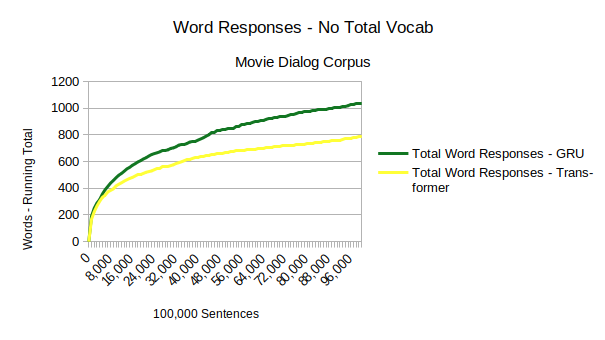
\includegraphics[scale=0.75]{diagram-100000-novocab}
		
		
	\end{center}
	\caption[Total Word Responses]{Total Word Responses - No Vocabulary Total}
	\label{diagram-words-no-voc-total}
	
\end{figure}

It is possible the GRU model operates more robustly than the Transformer model, or the Transformer model may be over trained or over fitted. It also might be that the hyper parameter set is poorly adjusted. The learning rate, for example, may be too high.

\subsection{Sentence Usage}
A goal for this work included answers to these questions.
How many fully formed responses does the given model use? Additionally, when or how many of these responses are used repeatedly?

While the GPT2 model is very large and very versatile, the Transformer and GRU models are smaller. In Figure \ref{diagram-words-limit-shown}, 100,000 inputs from the training set of the movie dialog corpus were used. 

The graph in Figure \ref{diagram-words-limit-shown} shows a running total of sentences used by the Transformer and the GRU. For every point on the $x$ axis, all sentences up to and including that index are fed to the Transformer and the GRU. At that point the graph shows a running total of sentences used more than once by the models, and how many sentences are used in total. These running totals are plotted on the $y$ axis of the graph.

These models use less than 2,000 sentences repeatedly. At the end of the study, 4,000 total sentences were used by the GRU. We feel that at some point the number of total GRU sentences that the model can produce will reach a limit below the vocabulary total.

\begin{figure}[H]
	\begin{center}
		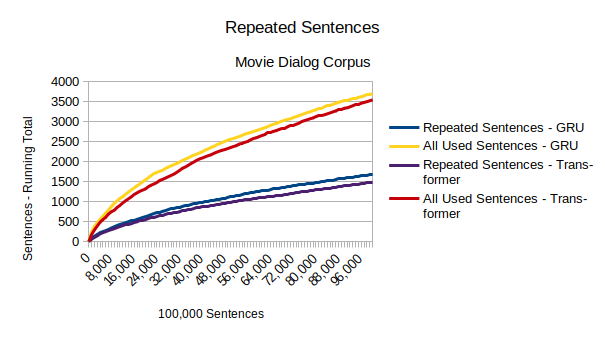
\includegraphics[scale=0.75]{diagram-100000-sent}
		
		
	\end{center}
	\caption[Simple Sentence Usage]{Simple Sentence Usage}
	\label{diagram-words-limit-shown}
	
\end{figure}

If the graphs of the repeated sentences changed vertically as they do horizontally, the lines would be shown to increase very slowly.

While the Transformer and GRU models have similar `Repeated Sentence' graphs, they are different models and have different sizes. 
However as they share the same corpus, they may be learning the same task.

\subsection{Maximum Sentence Values}

For each of the models there is only a certain number of tokens in the model's vocabulary. Additionally there are only so many tokens allowed in the output. For the GRU and the Transformer the output is limited to 10 tokens. For the GPT2 model there is a limit of 1024 tokens. There are only so many combinations that can be formed for a given model.

It seems that the models cannot use all of the words or tokens in their vocabulary. They can identify a number of them that they use repeatedly. This would mean the possible combinations that a model could produce is smaller.

\section{Training and Lists}

Here the Transformer and GRU models are trained on the movie dialog corpus. The Transformer model has 6 layers, 8 heads, and a hidden size of 512 units, while the GRU model has a hidden size of 500.

Initially the model learns a set of multi-purpose English answers. Then it acts as a classifier, where each input sentence is compared to the set of answers. There would be fewer answers than there are questions. 

At the start the multi-purpose answers are constructed at the same time that the classification task is taking place. 

The model has a certain capacity and it starts to develop lists of usable answers in order to use that capacity best.

For the GPT2, full sentences may not be saved because the model may be more dynamic. For translation, for instance, it may be able to remember longer lists. In place of a list of complete responses, a list of phrases or partial responses could be combined to create translated output.

The output of the Transformer or GRU shows little intelligence. The actual utterances of the model are plain. The internal building of lists, though, may show a process that is found in some intelligent activity.